% Graphic for TeX using PGF
% Title: /home/hayat/report_memoire/illustrations/graphe-nosql.dia
% Creator: Dia v0.97+git
% CreationDate: Sun Dec  2 17:45:15 2018
% For: hayat
% \usepackage{tikz}
% The following commands are not supported in PSTricks at present
% We define them conditionally, so when they are implemented,
% this pgf file will use them.
\ifx\du\undefined
  \newlength{\du}
\fi
\setlength{\du}{15\unitlength}
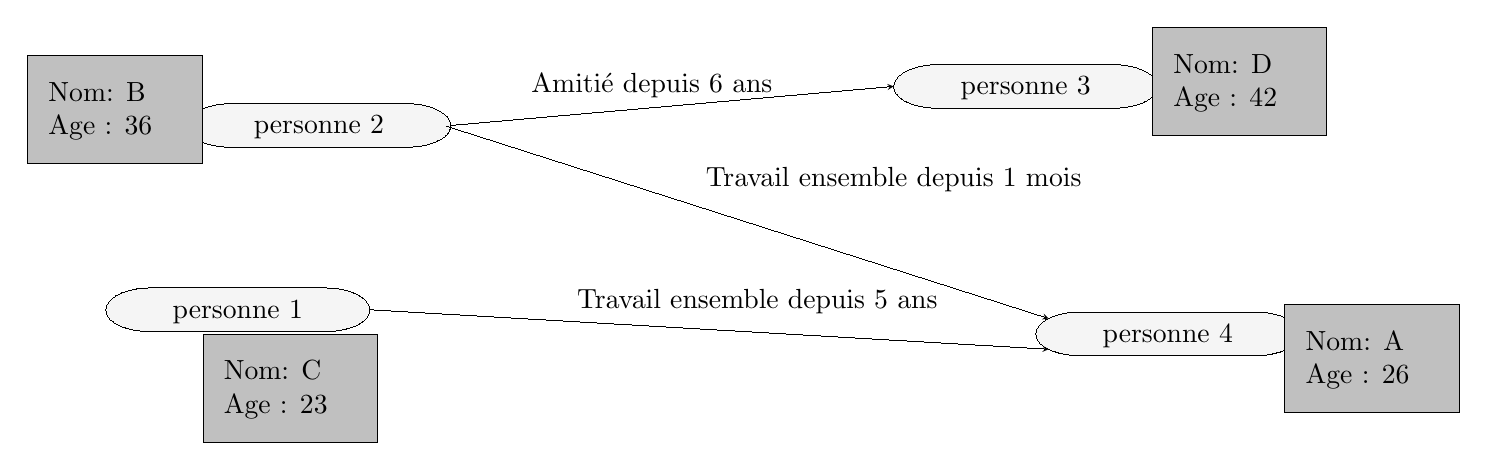
\begin{tikzpicture}[even odd rule]
\pgftransformxscale{1.000000}
\pgftransformyscale{-1.000000}
\definecolor{dialinecolor}{rgb}{0.000000, 0.000000, 0.000000}
\pgfsetstrokecolor{dialinecolor}
\pgfsetstrokeopacity{1.000000}
\definecolor{diafillcolor}{rgb}{1.000000, 1.000000, 1.000000}
\pgfsetfillcolor{diafillcolor}
\pgfsetfillopacity{1.000000}
\pgfsetlinewidth{0.000000\du}
\pgfsetdash{}{0pt}
\pgfsetbuttcap
\pgfsetmiterjoin
\pgfsetlinewidth{0.000000\du}
\pgfsetbuttcap
\pgfsetmiterjoin
\pgfsetdash{}{0pt}
\definecolor{diafillcolor}{rgb}{0.960784, 0.960784, 0.960784}
\pgfsetfillcolor{diafillcolor}
\pgfsetfillopacity{1.000000}
\definecolor{dialinecolor}{rgb}{0.000000, 0.000000, 0.000000}
\pgfsetstrokecolor{dialinecolor}
\pgfsetstrokeopacity{1.000000}
\pgfpathmoveto{\pgfpoint{3.655000\du}{7.600000\du}}
\pgfpathlineto{\pgfpoint{7.895000\du}{7.600000\du}}
\pgfpathcurveto{\pgfpoint{8.480422\du}{7.600000\du}}{\pgfpoint{8.955000\du}{7.835050\du}}{\pgfpoint{8.955000\du}{8.125000\du}}
\pgfpathcurveto{\pgfpoint{8.955000\du}{8.414950\du}}{\pgfpoint{8.480422\du}{8.650000\du}}{\pgfpoint{7.895000\du}{8.650000\du}}
\pgfpathlineto{\pgfpoint{3.655000\du}{8.650000\du}}
\pgfpathcurveto{\pgfpoint{3.069578\du}{8.650000\du}}{\pgfpoint{2.595000\du}{8.414950\du}}{\pgfpoint{2.595000\du}{8.125000\du}}
\pgfpathcurveto{\pgfpoint{2.595000\du}{7.835050\du}}{\pgfpoint{3.069578\du}{7.600000\du}}{\pgfpoint{3.655000\du}{7.600000\du}}
\pgfpathclose
\pgfusepath{fill,stroke}
% setfont left to latex
\definecolor{dialinecolor}{rgb}{0.000000, 0.000000, 0.000000}
\pgfsetstrokecolor{dialinecolor}
\pgfsetstrokeopacity{1.000000}
\definecolor{diafillcolor}{rgb}{0.000000, 0.000000, 0.000000}
\pgfsetfillcolor{diafillcolor}
\pgfsetfillopacity{1.000000}
\node[anchor=base,inner sep=0pt, outer sep=0pt,color=dialinecolor] at (5.775000\du,8.325000\du){personne 1};
\pgfsetlinewidth{0.000000\du}
\pgfsetdash{}{0pt}
\pgfsetbuttcap
\pgfsetmiterjoin
\pgfsetlinewidth{0.000000\du}
\pgfsetbuttcap
\pgfsetmiterjoin
\pgfsetdash{}{0pt}
\definecolor{diafillcolor}{rgb}{0.960784, 0.960784, 0.960784}
\pgfsetfillcolor{diafillcolor}
\pgfsetfillopacity{1.000000}
\definecolor{dialinecolor}{rgb}{0.000000, 0.000000, 0.000000}
\pgfsetstrokecolor{dialinecolor}
\pgfsetstrokeopacity{1.000000}
\pgfpathmoveto{\pgfpoint{5.608750\du}{3.160000\du}}
\pgfpathlineto{\pgfpoint{9.848750\du}{3.160000\du}}
\pgfpathcurveto{\pgfpoint{10.434172\du}{3.160000\du}}{\pgfpoint{10.908750\du}{3.395050\du}}{\pgfpoint{10.908750\du}{3.685000\du}}
\pgfpathcurveto{\pgfpoint{10.908750\du}{3.974950\du}}{\pgfpoint{10.434172\du}{4.210000\du}}{\pgfpoint{9.848750\du}{4.210000\du}}
\pgfpathlineto{\pgfpoint{5.608750\du}{4.210000\du}}
\pgfpathcurveto{\pgfpoint{5.023328\du}{4.210000\du}}{\pgfpoint{4.548750\du}{3.974950\du}}{\pgfpoint{4.548750\du}{3.685000\du}}
\pgfpathcurveto{\pgfpoint{4.548750\du}{3.395050\du}}{\pgfpoint{5.023328\du}{3.160000\du}}{\pgfpoint{5.608750\du}{3.160000\du}}
\pgfpathclose
\pgfusepath{fill,stroke}
% setfont left to latex
\definecolor{dialinecolor}{rgb}{0.000000, 0.000000, 0.000000}
\pgfsetstrokecolor{dialinecolor}
\pgfsetstrokeopacity{1.000000}
\definecolor{diafillcolor}{rgb}{0.000000, 0.000000, 0.000000}
\pgfsetfillcolor{diafillcolor}
\pgfsetfillopacity{1.000000}
\node[anchor=base,inner sep=0pt, outer sep=0pt,color=dialinecolor] at (7.728750\du,3.885000\du){personne 2};
\pgfsetlinewidth{0.000000\du}
\pgfsetdash{}{0pt}
\pgfsetbuttcap
\pgfsetmiterjoin
\pgfsetlinewidth{0.000000\du}
\pgfsetbuttcap
\pgfsetmiterjoin
\pgfsetdash{}{0pt}
\definecolor{diafillcolor}{rgb}{0.960784, 0.960784, 0.960784}
\pgfsetfillcolor{diafillcolor}
\pgfsetfillopacity{1.000000}
\definecolor{dialinecolor}{rgb}{0.000000, 0.000000, 0.000000}
\pgfsetstrokecolor{dialinecolor}
\pgfsetstrokeopacity{1.000000}
\pgfpathmoveto{\pgfpoint{22.633750\du}{2.220000\du}}
\pgfpathlineto{\pgfpoint{26.873750\du}{2.220000\du}}
\pgfpathcurveto{\pgfpoint{27.459172\du}{2.220000\du}}{\pgfpoint{27.933750\du}{2.455050\du}}{\pgfpoint{27.933750\du}{2.745000\du}}
\pgfpathcurveto{\pgfpoint{27.933750\du}{3.034950\du}}{\pgfpoint{27.459172\du}{3.270000\du}}{\pgfpoint{26.873750\du}{3.270000\du}}
\pgfpathlineto{\pgfpoint{22.633750\du}{3.270000\du}}
\pgfpathcurveto{\pgfpoint{22.048328\du}{3.270000\du}}{\pgfpoint{21.573750\du}{3.034950\du}}{\pgfpoint{21.573750\du}{2.745000\du}}
\pgfpathcurveto{\pgfpoint{21.573750\du}{2.455050\du}}{\pgfpoint{22.048328\du}{2.220000\du}}{\pgfpoint{22.633750\du}{2.220000\du}}
\pgfpathclose
\pgfusepath{fill,stroke}
% setfont left to latex
\definecolor{dialinecolor}{rgb}{0.000000, 0.000000, 0.000000}
\pgfsetstrokecolor{dialinecolor}
\pgfsetstrokeopacity{1.000000}
\definecolor{diafillcolor}{rgb}{0.000000, 0.000000, 0.000000}
\pgfsetfillcolor{diafillcolor}
\pgfsetfillopacity{1.000000}
\node[anchor=base,inner sep=0pt, outer sep=0pt,color=dialinecolor] at (24.753750\du,2.945000\du){personne 3};
\pgfsetlinewidth{0.000000\du}
\pgfsetdash{}{0pt}
\pgfsetbuttcap
\pgfsetmiterjoin
\pgfsetlinewidth{0.000000\du}
\pgfsetbuttcap
\pgfsetmiterjoin
\pgfsetdash{}{0pt}
\definecolor{diafillcolor}{rgb}{0.960784, 0.960784, 0.960784}
\pgfsetfillcolor{diafillcolor}
\pgfsetfillopacity{1.000000}
\definecolor{dialinecolor}{rgb}{0.000000, 0.000000, 0.000000}
\pgfsetstrokecolor{dialinecolor}
\pgfsetstrokeopacity{1.000000}
\pgfpathmoveto{\pgfpoint{26.058750\du}{8.180000\du}}
\pgfpathlineto{\pgfpoint{30.298750\du}{8.180000\du}}
\pgfpathcurveto{\pgfpoint{30.884172\du}{8.180000\du}}{\pgfpoint{31.358750\du}{8.415050\du}}{\pgfpoint{31.358750\du}{8.705000\du}}
\pgfpathcurveto{\pgfpoint{31.358750\du}{8.994950\du}}{\pgfpoint{30.884172\du}{9.230000\du}}{\pgfpoint{30.298750\du}{9.230000\du}}
\pgfpathlineto{\pgfpoint{26.058750\du}{9.230000\du}}
\pgfpathcurveto{\pgfpoint{25.473328\du}{9.230000\du}}{\pgfpoint{24.998750\du}{8.994950\du}}{\pgfpoint{24.998750\du}{8.705000\du}}
\pgfpathcurveto{\pgfpoint{24.998750\du}{8.415050\du}}{\pgfpoint{25.473328\du}{8.180000\du}}{\pgfpoint{26.058750\du}{8.180000\du}}
\pgfpathclose
\pgfusepath{fill,stroke}
% setfont left to latex
\definecolor{dialinecolor}{rgb}{0.000000, 0.000000, 0.000000}
\pgfsetstrokecolor{dialinecolor}
\pgfsetstrokeopacity{1.000000}
\definecolor{diafillcolor}{rgb}{0.000000, 0.000000, 0.000000}
\pgfsetfillcolor{diafillcolor}
\pgfsetfillopacity{1.000000}
\node[anchor=base,inner sep=0pt, outer sep=0pt,color=dialinecolor] at (28.178750\du,8.905000\du){personne 4};
\pgfsetlinewidth{0.000000\du}
\pgfsetdash{}{0pt}
\pgfsetbuttcap
{
\definecolor{diafillcolor}{rgb}{0.000000, 0.000000, 0.000000}
\pgfsetfillcolor{diafillcolor}
\pgfsetfillopacity{1.000000}
% was here!!!
\pgfsetarrowsend{stealth}
\definecolor{dialinecolor}{rgb}{0.000000, 0.000000, 0.000000}
\pgfsetstrokecolor{dialinecolor}
\pgfsetstrokeopacity{1.000000}
\draw (10.908750\du,3.685000\du)--(21.573750\du,2.745000\du);
}
% setfont left to latex
\definecolor{dialinecolor}{rgb}{0.000000, 0.000000, 0.000000}
\pgfsetstrokecolor{dialinecolor}
\pgfsetstrokeopacity{1.000000}
\definecolor{diafillcolor}{rgb}{0.000000, 0.000000, 0.000000}
\pgfsetfillcolor{diafillcolor}
\pgfsetfillopacity{1.000000}
\node[anchor=base west,inner sep=0pt,outer sep=0pt,color=dialinecolor] at (12.850000\du,2.900000\du){Amitié depuis 6 ans};
\pgfsetlinewidth{0.000000\du}
\pgfsetdash{}{0pt}
\pgfsetbuttcap
{
\definecolor{diafillcolor}{rgb}{0.000000, 0.000000, 0.000000}
\pgfsetfillcolor{diafillcolor}
\pgfsetfillopacity{1.000000}
% was here!!!
\pgfsetarrowsend{stealth}
\definecolor{dialinecolor}{rgb}{0.000000, 0.000000, 0.000000}
\pgfsetstrokecolor{dialinecolor}
\pgfsetstrokeopacity{1.000000}
\draw (8.955000\du,8.125000\du)--(25.309224\du,9.076227\du);
}
% setfont left to latex
\definecolor{dialinecolor}{rgb}{0.000000, 0.000000, 0.000000}
\pgfsetstrokecolor{dialinecolor}
\pgfsetstrokeopacity{1.000000}
\definecolor{diafillcolor}{rgb}{0.000000, 0.000000, 0.000000}
\pgfsetfillcolor{diafillcolor}
\pgfsetfillopacity{1.000000}
\node[anchor=base west,inner sep=0pt,outer sep=0pt,color=dialinecolor] at (13.950000\du,8.100000\du){Travail ensemble depuis 5 ans};
\pgfsetlinewidth{0.000000\du}
\pgfsetdash{}{0pt}
\pgfsetbuttcap
{
\definecolor{diafillcolor}{rgb}{0.000000, 0.000000, 0.000000}
\pgfsetfillcolor{diafillcolor}
\pgfsetfillopacity{1.000000}
% was here!!!
\pgfsetarrowsend{stealth}
\definecolor{dialinecolor}{rgb}{0.000000, 0.000000, 0.000000}
\pgfsetstrokecolor{dialinecolor}
\pgfsetstrokeopacity{1.000000}
\draw (10.800000\du,3.700000\du)--(25.309224\du,8.333773\du);
}
% setfont left to latex
\definecolor{dialinecolor}{rgb}{0.000000, 0.000000, 0.000000}
\pgfsetstrokecolor{dialinecolor}
\pgfsetstrokeopacity{1.000000}
\definecolor{diafillcolor}{rgb}{0.000000, 0.000000, 0.000000}
\pgfsetfillcolor{diafillcolor}
\pgfsetfillopacity{1.000000}
\node[anchor=base west,inner sep=0pt,outer sep=0pt,color=dialinecolor] at (17.050000\du,5.150000\du){Travail ensemble depuis 1 mois};
\pgfsetlinewidth{0.000000\du}
\pgfsetdash{}{0pt}
\pgfsetmiterjoin
{\pgfsetcornersarced{\pgfpoint{0.000000\du}{0.000000\du}}\definecolor{diafillcolor}{rgb}{0.752941, 0.752941, 0.752941}
\pgfsetfillcolor{diafillcolor}
\pgfsetfillopacity{1.000000}
\fill (31.000050\du,8.000000\du)--(31.000050\du,10.600000\du)--(35.200050\du,10.600000\du)--(35.200050\du,8.000000\du)--cycle;
}{\pgfsetcornersarced{\pgfpoint{0.000000\du}{0.000000\du}}\definecolor{dialinecolor}{rgb}{0.000000, 0.000000, 0.000000}
\pgfsetstrokecolor{dialinecolor}
\pgfsetstrokeopacity{1.000000}
\draw (31.000050\du,8.000000\du)--(31.000050\du,10.600000\du)--(35.200050\du,10.600000\du)--(35.200050\du,8.000000\du)--cycle;
}% setfont left to latex
\definecolor{dialinecolor}{rgb}{0.000000, 0.000000, 0.000000}
\pgfsetstrokecolor{dialinecolor}
\pgfsetstrokeopacity{1.000000}
\definecolor{diafillcolor}{rgb}{0.000000, 0.000000, 0.000000}
\pgfsetfillcolor{diafillcolor}
\pgfsetfillopacity{1.000000}
\node[anchor=base west,inner sep=0pt,outer sep=0pt,color=dialinecolor] at (31.500050\du,9.095000\du){Nom: A};
% setfont left to latex
\definecolor{dialinecolor}{rgb}{0.000000, 0.000000, 0.000000}
\pgfsetstrokecolor{dialinecolor}
\pgfsetstrokeopacity{1.000000}
\definecolor{diafillcolor}{rgb}{0.000000, 0.000000, 0.000000}
\pgfsetfillcolor{diafillcolor}
\pgfsetfillopacity{1.000000}
\node[anchor=base west,inner sep=0pt,outer sep=0pt,color=dialinecolor] at (31.500050\du,9.895000\du){Age : 26 };
\pgfsetlinewidth{0.000000\du}
\pgfsetdash{}{0pt}
\pgfsetmiterjoin
{\pgfsetcornersarced{\pgfpoint{0.000000\du}{0.000000\du}}\definecolor{diafillcolor}{rgb}{0.752941, 0.752941, 0.752941}
\pgfsetfillcolor{diafillcolor}
\pgfsetfillopacity{1.000000}
\fill (0.713750\du,2.010000\du)--(0.713750\du,4.610000\du)--(4.913750\du,4.610000\du)--(4.913750\du,2.010000\du)--cycle;
}{\pgfsetcornersarced{\pgfpoint{0.000000\du}{0.000000\du}}\definecolor{dialinecolor}{rgb}{0.000000, 0.000000, 0.000000}
\pgfsetstrokecolor{dialinecolor}
\pgfsetstrokeopacity{1.000000}
\draw (0.713750\du,2.010000\du)--(0.713750\du,4.610000\du)--(4.913750\du,4.610000\du)--(4.913750\du,2.010000\du)--cycle;
}% setfont left to latex
\definecolor{dialinecolor}{rgb}{0.000000, 0.000000, 0.000000}
\pgfsetstrokecolor{dialinecolor}
\pgfsetstrokeopacity{1.000000}
\definecolor{diafillcolor}{rgb}{0.000000, 0.000000, 0.000000}
\pgfsetfillcolor{diafillcolor}
\pgfsetfillopacity{1.000000}
\node[anchor=base west,inner sep=0pt,outer sep=0pt,color=dialinecolor] at (1.213750\du,3.105000\du){Nom: B};
% setfont left to latex
\definecolor{dialinecolor}{rgb}{0.000000, 0.000000, 0.000000}
\pgfsetstrokecolor{dialinecolor}
\pgfsetstrokeopacity{1.000000}
\definecolor{diafillcolor}{rgb}{0.000000, 0.000000, 0.000000}
\pgfsetfillcolor{diafillcolor}
\pgfsetfillopacity{1.000000}
\node[anchor=base west,inner sep=0pt,outer sep=0pt,color=dialinecolor] at (1.213750\du,3.905000\du){Age : 36 };
\pgfsetlinewidth{0.000000\du}
\pgfsetdash{}{0pt}
\pgfsetmiterjoin
{\pgfsetcornersarced{\pgfpoint{0.000000\du}{0.000000\du}}\definecolor{diafillcolor}{rgb}{0.752941, 0.752941, 0.752941}
\pgfsetfillcolor{diafillcolor}
\pgfsetfillopacity{1.000000}
\fill (4.938750\du,8.720000\du)--(4.938750\du,11.320000\du)--(9.138750\du,11.320000\du)--(9.138750\du,8.720000\du)--cycle;
}{\pgfsetcornersarced{\pgfpoint{0.000000\du}{0.000000\du}}\definecolor{dialinecolor}{rgb}{0.000000, 0.000000, 0.000000}
\pgfsetstrokecolor{dialinecolor}
\pgfsetstrokeopacity{1.000000}
\draw (4.938750\du,8.720000\du)--(4.938750\du,11.320000\du)--(9.138750\du,11.320000\du)--(9.138750\du,8.720000\du)--cycle;
}% setfont left to latex
\definecolor{dialinecolor}{rgb}{0.000000, 0.000000, 0.000000}
\pgfsetstrokecolor{dialinecolor}
\pgfsetstrokeopacity{1.000000}
\definecolor{diafillcolor}{rgb}{0.000000, 0.000000, 0.000000}
\pgfsetfillcolor{diafillcolor}
\pgfsetfillopacity{1.000000}
\node[anchor=base west,inner sep=0pt,outer sep=0pt,color=dialinecolor] at (5.438750\du,9.815000\du){Nom: C};
% setfont left to latex
\definecolor{dialinecolor}{rgb}{0.000000, 0.000000, 0.000000}
\pgfsetstrokecolor{dialinecolor}
\pgfsetstrokeopacity{1.000000}
\definecolor{diafillcolor}{rgb}{0.000000, 0.000000, 0.000000}
\pgfsetfillcolor{diafillcolor}
\pgfsetfillopacity{1.000000}
\node[anchor=base west,inner sep=0pt,outer sep=0pt,color=dialinecolor] at (5.438750\du,10.615000\du){Age : 23 };
\pgfsetlinewidth{0.000000\du}
\pgfsetdash{}{0pt}
\pgfsetmiterjoin
{\pgfsetcornersarced{\pgfpoint{0.000000\du}{0.000000\du}}\definecolor{diafillcolor}{rgb}{0.752941, 0.752941, 0.752941}
\pgfsetfillcolor{diafillcolor}
\pgfsetfillopacity{1.000000}
\fill (27.813750\du,1.330000\du)--(27.813750\du,3.930000\du)--(32.013750\du,3.930000\du)--(32.013750\du,1.330000\du)--cycle;
}{\pgfsetcornersarced{\pgfpoint{0.000000\du}{0.000000\du}}\definecolor{dialinecolor}{rgb}{0.000000, 0.000000, 0.000000}
\pgfsetstrokecolor{dialinecolor}
\pgfsetstrokeopacity{1.000000}
\draw (27.813750\du,1.330000\du)--(27.813750\du,3.930000\du)--(32.013750\du,3.930000\du)--(32.013750\du,1.330000\du)--cycle;
}% setfont left to latex
\definecolor{dialinecolor}{rgb}{0.000000, 0.000000, 0.000000}
\pgfsetstrokecolor{dialinecolor}
\pgfsetstrokeopacity{1.000000}
\definecolor{diafillcolor}{rgb}{0.000000, 0.000000, 0.000000}
\pgfsetfillcolor{diafillcolor}
\pgfsetfillopacity{1.000000}
\node[anchor=base west,inner sep=0pt,outer sep=0pt,color=dialinecolor] at (28.313750\du,2.425000\du){Nom: D};
% setfont left to latex
\definecolor{dialinecolor}{rgb}{0.000000, 0.000000, 0.000000}
\pgfsetstrokecolor{dialinecolor}
\pgfsetstrokeopacity{1.000000}
\definecolor{diafillcolor}{rgb}{0.000000, 0.000000, 0.000000}
\pgfsetfillcolor{diafillcolor}
\pgfsetfillopacity{1.000000}
\node[anchor=base west,inner sep=0pt,outer sep=0pt,color=dialinecolor] at (28.313750\du,3.225000\du){Age : 42 };
\end{tikzpicture}
